%---------------------------------------------------------------------------
% スタイル定義.kaisetsu, jikkennsitsu, topics, salonのどれかを選ぶ.
%---------------------------------------------------------------------------
%\documentclass[kaisetsu,b5paper,papersize,twocolumn]{jsarticle}
%\documentclass[jikkensitsu,b5paper,papersize,twocolumn]{jsarticle}
\documentclass[topics,b5paper,papersize,twocolumn]{jsarticle}
%\documentclass[salon, b5paper,papersize,twocolumn]{jsarticle}
%---------------------------------------------------------------------------

\usepackage{kotaibutsuri}
\usepackage{mediabb}
\usepackage[hyphens]{url}
\usepackage{graphicx}

\title{急減圧液体における気泡のオストワルド成長}
%\subtitle{サブタイトル}

\author{渡辺宙志}
\affiliation{東京大学物性研究所附属物質設計評価施設}

\startpage{33}
\starttotalpage{100}
\articlevolume{53}
\articlenumber{3}
\articleyear{2018}

\newcommand{\diff}{\mathrm{d}}

\begin{document}
\maketitle

\section{はじめに}

合金系を一度高温にしてから転移温度以下に保持すると,相分離により結晶成長が起きる.
この時,最初は小さな結晶核が多数発生するが,そのうち大きな結晶がより大きく,小さな結晶がより小さくなっていく現象が起きる.
この「富めるものはより富み,貧しいものはより貧しくなる」現象はオストワルド成長(Ostwald Ripening)と呼ばれている.
オストワルド成長は一次転移を引き起こす系で普遍的に見られるが,その工学応用上の重要性から,主に溶液からの固体の析出や合金系の相分離の枠組みにおいて研究が盛んに行われてきた\cite{Baldan}.
合金系におけるオストワルド成長は,結晶核がそのサイズによって融点が変わるギブス・トムソン効果により
説明されることが多いが,本質的には系が全体の界面自由エネルギーを減らそうとすることによって起きる現象である.
身近なオストワルド成長の例としては,石灰岩が熱変成をうけて大理石になったり,アイスクリームを冷凍庫で長期間保存すると,氷の結晶が成長することで風味が落ちることなどが挙げられる\cite{ice}.ストローの左右に大きさの異なるシャボン玉をつけると,小さい方が圧力が高いためにしぼんでいき,最終的にどちらか片方のシャボン玉のみになるが,これも大きく捉えればオストワルド成長と同様な原理とみなせる.
オストワルド成長を理論的に記述する試みは古くからあるが,1960年代に入って
Lifshitz-Slyozov,そしてWagnerらによるスケーリングの概念の導入により古典論として完成する\cite{LS,Wagner}.
このオストワルド成長の古典論は,三人の名をとってLSW理論と呼ばれている\footnote{
余談であるが,Lifshitz-Slyozov (LS)の原著論文はロシア語,Wagnerの原著論文はドイツ語である.
LSの論文は英訳されており,引用されるのはほぼ英訳版だが,Wagnerの論文は英訳が無く,ドイツ語版が引用されている.
筆者はちゃんとドイツ語版を読んだことは主張しておきたい.
}.
さて,LSW理論は準安定状態から平衡状態にいたる緩和過程を記述する理論であるが,
同じく準安定状態にある系を扱いつつ,非平衡定常状態を記述するのが古典核生成論と呼ばれる理論である.
古典核生成論は,準安定状態にある系から核が生成し,成長していく過程を記述する理論であり,
例えば過飽和蒸気における液滴生成率などを予言することができる.
準安定状態からの緩和は1870年代からGibbsらによって記述されているが\cite{Gibbs},
現在,古典核生成論と呼ばれるものは,1920年代から40年代にかけて構築されたものである\cite{CNT}.
古典核生成論は,表式上は一次転移一般に適用できる理論であるが,液滴生成率の予言ではオーダーは合うものの\cite{Horsch},
液滴生成と相転移の表裏である気泡生成では,気泡生成率を実験値より何桁も小さく見積もってしまう\cite{Vinogradov}.
この傾向は数値計算でも同様であり,数値計算で求められる気泡生成率より古典核生成論による予言は何桁も小さい\cite{Zeng, Yamamoto, wtime}.
この不一致の原因がなんであるかが長らく問題となっていた.
そこで我々は,京コンピュータを使って急減圧した液体中に発生する多数の気泡によるオストワルド成長を観測し,その振る舞いをLSW理論を用いて解析した.計算の目的は,気泡成長のスケーリングを観察することでミクロな気泡のダイナミクスを調べ,「なぜ古典論がなぜ気泡生成率の予言に失敗するか」を調べることであった.
本稿では,古典核生成論とLSW理論の関係や,なぜ古典核生成論を検証するのにLSW理論を用いたのかなどについて紹介する.
また,本研究の広報を通じて得た思わぬ知見についても併せて紹介したい.

\section{古典核生成論とLSW理論}

\subsection{古典核生成論}

\begin{figure}[tb]
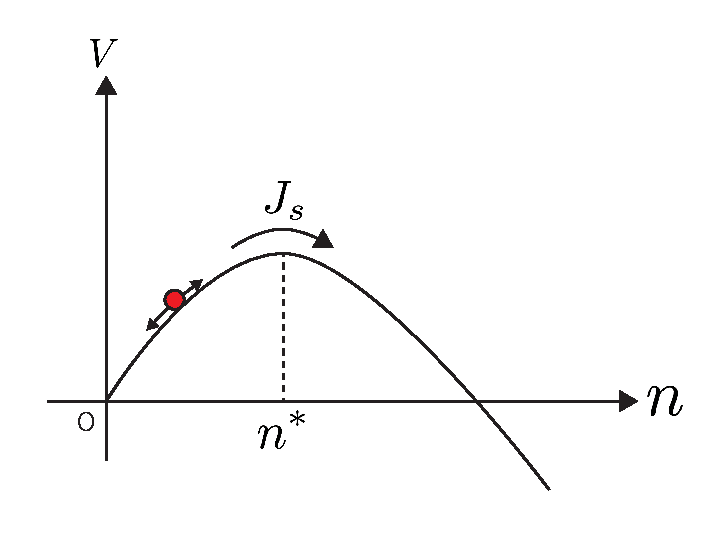
\includegraphics[width=0.8\linewidth]{rw.pdf}
\caption{核生成率.系は分子数$n$に関するランダムウォークで記述される\cite{CNT}.
界面自由エネルギーと化学ポテンシャル差のバランスから決まる臨界サイズ$n^*$をピークとする
エネルギーバリアがあり,そのバリアを超えた液滴は成長する一方となる.単位時間,単位体積あたりに
そのバリアを超える液滴の数が液滴の核生成率$J_s$である.
}\label{fig_rw}
\end{figure}

一次転移を引き起こす系の外場を急に変化させると系が準安定状態となる.
準安定状態から安定状態に緩和する際,安定相が核として生成し,成長していくが,
この核生成のダイナミクスを記述するのが古典核生成論(Classical Nucleation Theory, CNT)である.
今日,いわゆる古典核生成論と呼ばれる理論は1900年代前半にFarkasやZeldovichによってまとめられたものである\cite{Farkas, Zeldovich}.以下,過飽和蒸気中の液滴生成を例として,古典核生成論を簡単に導出する\footnote{
気泡生成の場合には,気泡が成長する際に液相にする仕事も考慮する必要がある\cite{Blander}.
}.
ある時刻$t$において,内部に$n$個の分子を含む液滴クラスターの個数を$f(n,t)$としよう.
さらに$n$個の分子を含む液滴クラスターの,単位時間あたり分子を一つ獲得する確率を$W_+(n)$,
一つ放出する確率を$W_-(n)$とする.いま,分子の放出及び獲得は一度に一つずつしか行われないと仮定すると,$f(n,t)$に関するマスター方程式は
\begin{align}
\frac{\partial f}{\partial t} &= 
-\left[ W_+(n) + W_-(n)\right] f(n,t) \nonumber \\
&+ W_+(n-1)f(n-1,t)  \nonumber \\
&+ W_-(n+1)f(n+1,t)
\end{align}
と書ける.
平衡状態におけるクラスター数分布を$f_0(n)$とすると,詳細釣合の条件から
\begin{equation}
W_+ f_0(n) = W_- f_0(n+1)
\end{equation}
が成立する.ここから$W_-$を消去し,さらに$n$に関して連続近似をすると
\begin{equation}
\frac{\partial f}{\partial t} = - \frac{\partial}{\partial n}
\left(
\displaystyle \frac{W_+}{f_0} \frac{\partial f_0}{\partial n}
- W_+ \frac{\partial}{\partial n}
\right) f
\label{eq_c}
\end{equation}
を得る.
いま,系は過飽和であるから,気体であるよりも液体であった方が自由エネルギーが低い.
しかし,液滴が生成されると,界面自由エネルギーの分だけ損をする.
従って,ある臨界サイズ$n^*$が存在し,その臨界サイズより小さいクラスターはより小さく,
臨界サイズ以上のクラスターは大きくなりやすいことが予想される.
従って式(\ref{eq_c})は,分子数$n$を位置とみなすと,ある臨界サイズ$n^*$までは上り坂,それを超えるとあとは下り坂
となるようなポテンシャル下におけるランダムウォークを記述している(\textbf{第\ref{fig_rw}図}参照).

さて,系の過飽和度を固定しよう.大きく成長した液滴が(重力で落ちるなどして)取り除かれると思えば,系は定常状態となる.
この時,単位時間,単位体積あたりに臨界サイズ$n^*$をまたぐクラスターの数が
液滴の核生成率$J_s$であり,それを予言するのが古典核生成論である.
式(\ref{eq_c})は,時刻$t$と分子数$n$に依存する非線形偏微分方程式となっていたが,
定常状態を仮定することで$t$に関する自由度が落ちて常微分方程式となるため,解析的に$J_s$を評価できる.
計算の詳細は省くが,最終的に古典核生成論は核生成率を
\begin{equation}
J_s = Z W_+(n^*) f_0(n^*)
\end{equation}
と予言する.
$Z$はZeldovich定数と呼ばれる定数であり,式を$n^*$のまわりで鞍点近似する際に出てくる,
系の非平衡性を反映する物理量である.
$W_+(n)$や$f_0(n)$は平衡状態における物理量であり,$Z$も平衡状態の物性から求められるため,
平衡状態の性質から過飽和蒸気における液滴生成率が求められることになる.

\subsection{LSW理論}

次に,オストワルド成長の古典論,Lifshitz-Slyozov-Wagner (LSW)理論を紹介する.
後で見るようにLSW理論は古典核生成論と兄弟のような関係にある.
古典核生成論と同様に液滴生成を例にとろう.
内部に$n$個の分子を持つ液滴の数を$f(n,t)$とする.
オストワルド成長においても臨界サイズ$n^*$が存在し,それより大きな液滴は成長し,そうでない液滴は小さくなっていく.
定常状態を記述する古典核生成論とは異なり,その臨界サイズは時刻とともに大きくなっていく.ここで,その臨界サイズの漸近系が
\begin{equation}
n^* \sim t^x
\end{equation}
とベキ的に振る舞うことを仮定し,スケールされたサイズ$\tilde{n}=n/n^*$による表示により
分布関数が
\begin{equation}
f(n,t) \sim t^y \tilde{f}(\tilde{n}) \label{eq_continuous}
\end{equation}
とスケールできることを要請する\cite{Binder}.この分布関数は以下の連続の式に従うであろう.
\begin{equation}
\frac{\partial f}{\partial t}=-\frac{\partial}{\partial n}(\dot{n} f)
\end{equation}
ここで$\dot{n}(n,t)$はサイズ$n$の液滴の成長率である.この成長率も
\begin{equation}
\dot{n} \sim n^z \tilde{\dot{n}}(\tilde{n})
\end{equation}
とスケールすることを要請しよう.

\begin{figure*}[htbp]
\centering
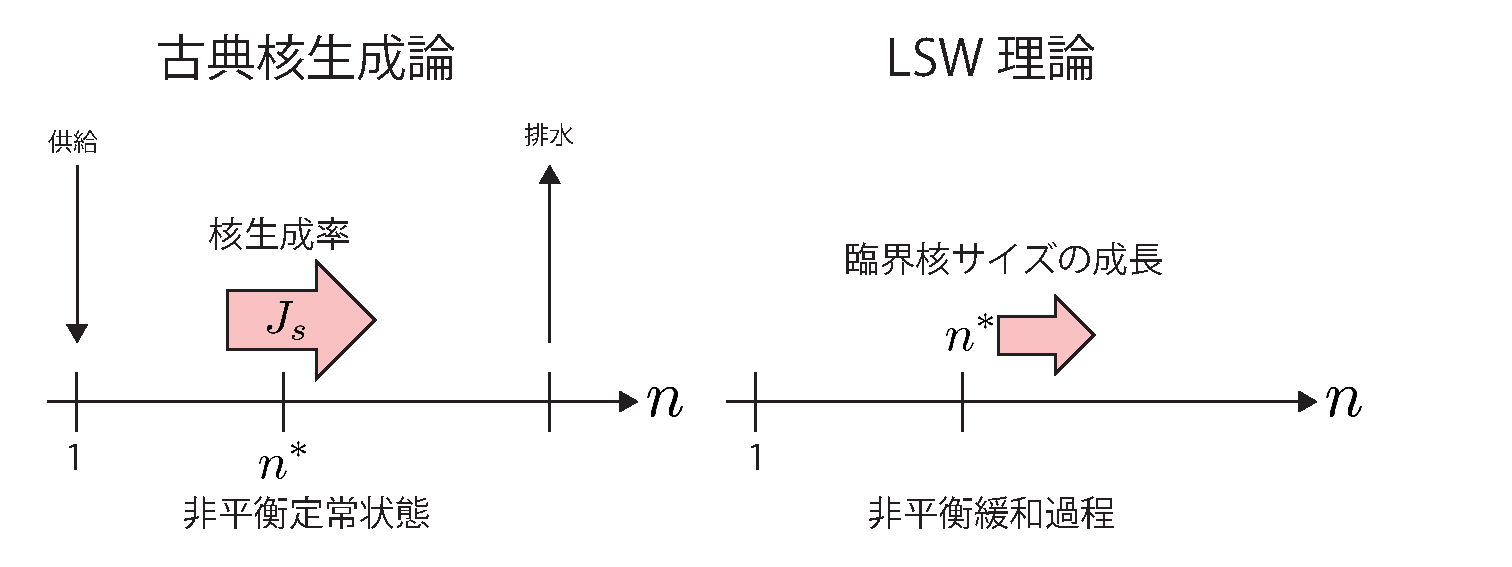
\includegraphics[width=0.7\linewidth]{compare.pdf}
\caption{
古典核生成論とLSW理論の構造.どちらも同じポテンシャル下でのランダムウォークであるが,
古典核生成論は興味あるサイズの両端の境界条件を固定することで定常状態とする\cite{CNT}.
LSW理論は自由境界条件を採用するが,スケーリングを仮定することで変数を一つ落としている\cite{Binder}.
古典核生成論では臨界サイズは時間変化せず,LSW理論では臨界サイズは時間とともに成長する.
}\label{fig_compare}
\end{figure*}

体積変化を伴うダイナミクスに比べて表面積変化のダイナミクスの方が遅いため,オストワルド成長の
後期過程においては液相の全体積はほとんど変化せず,液滴の全表面積のみ減っていくと考えられる.
液相の全体積は,分布関数の一次のモーメント
\begin{equation}
V_\mathrm{liquid} = \int n f(n,t) \diff n
\end{equation}
で与えられるが,これが時間変化しないことを要請すると,スケーリング関係式$y = -2 x$を得る.
さらに,スケールされた変数$\tilde{n}$や分布関数$\tilde{f}$で記述された連続の式(\ref{eq_continuous})も
時間に依存しないことを要請すると$z = x -1$が導かれる.以上から,ただ一つのスケーリング指数$x$によって
系の振る舞いが支配されていることがわかる.さらに,系に存在する液滴の数$N(t)$の漸近的な振る舞いが,
\begin{equation}
N(t) = \int f(n,t) \diff n \sim t^{-x}
\end{equation}
と,ベキ的に減衰することもわかる.

この指数$x$の値は液滴成長率$\dot{n}$の関数形に依存して決まる.
液滴が成長するには,外界から分子(モノマー)が供給され,かつそれが界面に吸着しなければならない.
界面での反応速度が早い極限では,分子の供給が律速となる(拡散律速).
逆に,界面での反応速度が遅い極限では,界面での吸着が律速となる(反応律速).
詳細は省くが,界面における拡散と反応の釣り合いの式を導出し,それぞれの極限をとることで,
拡散律速の場合には$x = 1$,反応律速の場合には$x = 3/2$となることを
示すことができる\footnote{この時,臨界核半径がそれぞれ$t^{1/3}$,$t^{1/2}$と振る舞うため,
それぞれ$1/3$則,$1/2$則と呼ばれている.}.
スケールされた連続の式は$\tilde{n}$に関する常微分方程式となるから,それぞれの極限において
スケールされた分布関数$\tilde{f}$も解析的に求めることができる.これがLSW理論である.

\subsection{古典核生成論とLSW理論の関係}

古典核生成論とLSW理論は同じ連続の式を異なる境界条件で解くことに対応している(\textbf{第\ref{fig_compare}図}参照).
連続の式は液滴のサイズと時間の二変数に依存しているが,古典核生成論は
定常状態を仮定することで$t$を落とし,LSW理論はスケーリングを仮定することで一変数に落としている.
さて,古典核生成論の構築において,いくつか重要な仮定が置かれていた.
まず,クラスター数分布$f(n,t)$が,時刻$t$と分子数$n$にのみ依存するという仮定は,
ダイナミクスが履歴に依存しないことを要請する(マルコフ性).
さらに,マスター方程式を構成する上でクラスターの成長速度のみに注目しており,
クラスター同士の合体や,クラスターの分離など,クラスター間の相互作用は考慮されていない(平均場近似).
また,クラスターのダイナミクスを記述する係数$W_+(n)$や$W_-(n)$が,平衡状態と同じ関数形を持っている
という仮定も置かれている(弱非平衡近似).
古典核生成論が気泡生成率の予言に失敗する理由の解明のため,例えば多体効果を摂動的に取り入れるなどの改良も試みられているが,
たとえ実験値に合う値が出たとしても,本当にその近似が悪さをしていたのかの検討は不十分であった.
分子動力学法で気泡生成現象を再現すれば,少なくとも相転移と気泡間相互作用については近似なしに扱うことができるが,
古典核生成論が仮定する非平衡定常状態を数値計算で実現するのは難しい.

\begin{figure*}[tb]
\includegraphics[width=0.3\linewidth]{bubble1.jpg}
\includegraphics[width=0.3\linewidth]{bubble2.jpg}
\includegraphics[width=0.3\linewidth]{bubble3.jpg}
\caption{
多重気泡生成過程におけるオストワルド成長.多数の気泡が発生した後,大きな気泡はより大きく,小さな気泡はより小さくなり,最終的に大きな気泡一つに収束する.なお,合体イベントはほとんどおきず,気泡は圧力を介してのみ相互作用する.可視化は理研AICSの稲岡氏による\cite{Watanabe2014}.
}
\label{fig_bubble}
\end{figure*}

一方,LSW理論も平均場近似であり,液滴の成長率は平衡状態のものを使う(弱非平衡近似),
液滴の相互作用は無視する(平均場近似)など,そのほとんどの仮定を古典核生成論と共有している.
我々は古典核生成論が気泡生成を正しく記述できない主な原因は,多体効果を無視していることにあると考えていた.
水蒸気の中で浮かぶ液滴間の相互作用に比べて,液体の中に浮かぶ気泡間の相互作用は明らかに強い.
液滴間の相互作用が拡散でしか届かないのに対し,気泡間の相互作用は音速で届くため,時間スケールの分離もできない.
従って,多重気泡生成後のオストワルド成長過程は,LSW理論では正しく記述できないであろう,というのが我々の予想であった.
LSW理論が記述するのは非平衡緩和過程であり,気泡を生成させた後は孤立系として扱えるため数値的な取り扱いが容易である.
ただし,多重気泡生成過程を原子スケールから再現するには大規模な系が必要となる.
そこで我々は,計算規模の問題については大規模並列コードを開発することで力任せに解決し,
計算の条件に関しては,より実現が容易な非平衡非定常過程を観察することで,古典核生成論の問題を別の方向から検討することにした.

\section{気泡成長のスケーリング}

我々はLSW理論における平均場近似の妥当性を検証を目的とし,分子動力学計算を行った.
気泡界面の相転移から,気泡間の相互作用まで全てあらわに扱うため,計算は大規模なものが求められる.
事前の準備的計算により,気泡一つを再現するのに十万から百万原子程度必要であり,
多数の気泡が相互作用する状況を表現するには最低でも数億原子は必要であることがわかっていた.
この規模の計算となると並列化は必須となる.並列化にはMPIを用いたプロセス並列や
OpenMPを用いたスレッド並列などがあるが,この規模の計算では両者を併用した
ハイブリッド並列計算が必要になる.
我々は新たに大規模並列分子動力学計算コードを開発した\cite{mdacp,mdnote}.
疑似flat-MPI法という手法を開発し,さらに「京」向けに計算カーネルをチューニングすることで,
「京」フルノードで3318億原子のベンチマーク計算を実行,2.44ペタフロップス(ピーク性能比23\%)を達成した.
気泡生成のプロダクトランでも「京」フルノード137億原子の計算で,ピーク性能比17\%を達成した\cite{fx10full}.「京」においてチューニング不足のコードではピーク性能比で数\%出れば御の字であり,またベンチマークでは高性能が出せてもプロダクトランでは性能が落ちることが多いなか,これは高い数字である.
このコードを用いて,「京」4096ノードで7億粒子規模の多重気泡生成過程の計算を実行した\cite{Watanabe2014}.
まず系を液相に緩和させておき,あるとき一様に膨脹させることで減圧し,気泡を生成させる.
その後は気泡間相互作用によりオストワルド成長が観測された(\textbf{第\ref{fig_bubble}図}).

オストワルド成長により,気泡の数は時間経過にともなって減っていく.その減少のベキは系の律速によって決まる.
\textbf{第\ref{fig_result}図}に,気泡数の時間発展の温度依存性を示す.低温,高温の二つの結果が掲載されているが,
どちらも急減圧直後は気泡数が急激に増え,その後ベキ的に減少していることがわかる.
その振る舞いは,低温では$t^{-3/2}$,高温では$t^{-1}$であり,
緩和の指数からそれぞれ反応律速,拡散律速であることが予想される.

\begin{figure}[tb]
\centering
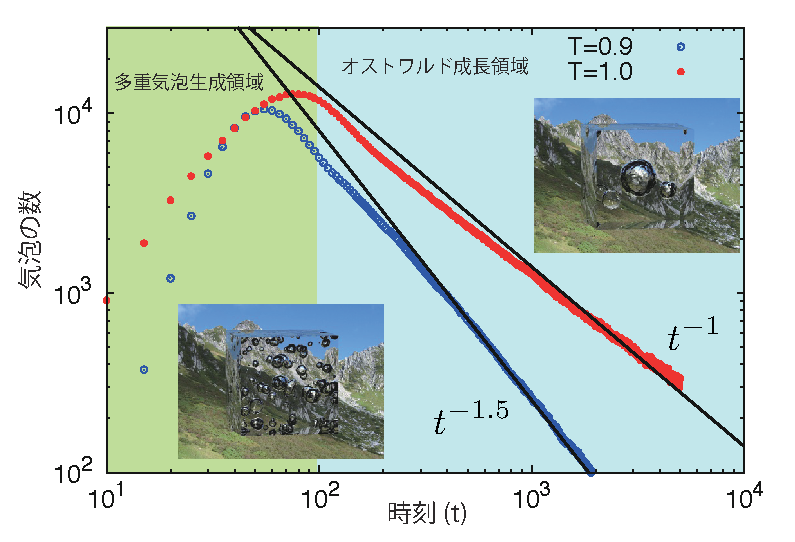
\includegraphics[width=0.9\linewidth]{result.pdf}
\caption{
気泡数の時間発展の温度依存性.最初に気泡数が増える時間領域(多重気泡生成領域)があり,
その後ベキ的に現象する時間領域(オストワルド成長領域)が存在する\cite{Watanabe2014}.
}\label{fig_result}
\end{figure}

さて,異なる時刻において,同じ位置にある気泡を同じ気泡とみなすと,個々の気泡の大きさの時間発展を追うことができる.
その情報から,ある時刻における気泡の成長率を計算することができる.成長率が正であれば気泡は膨張しており,
負であれば収縮していることを表す.\textbf{第\ref{fig_vdot}図}に低温領域における気泡の成長率のスケーリングを示す\cite{Watanabe2016}.
スケールされた体積$\tilde{v}$は,気泡体積$v$を臨界サイズ$v^*(t)$で割ったものであり,
$\tilde{v} = 1$の時に,気泡成長率はゼロとなる.
異なる時刻における気泡成長率が良くスケールされ,かつ反応律速の場合の理論曲線(実線)によく一致していることがわかる.
もし同時刻の気泡が異なる圧力を感じていた場合,気泡成長率は多値となり,この線はぼやけるはずである.
しかし,きれいに一つの直線にのっていることから,これは全ての気泡が同じ圧力を感じていること,すなわち
平均場描像が良い近似となっていることの直接的な証左となっている.
これらの結果は,気泡系におけるオストワルド成長が古典的なLSW理論でほぼ完全に記述されていることを示唆する.

\begin{figure}[tb]
\centering
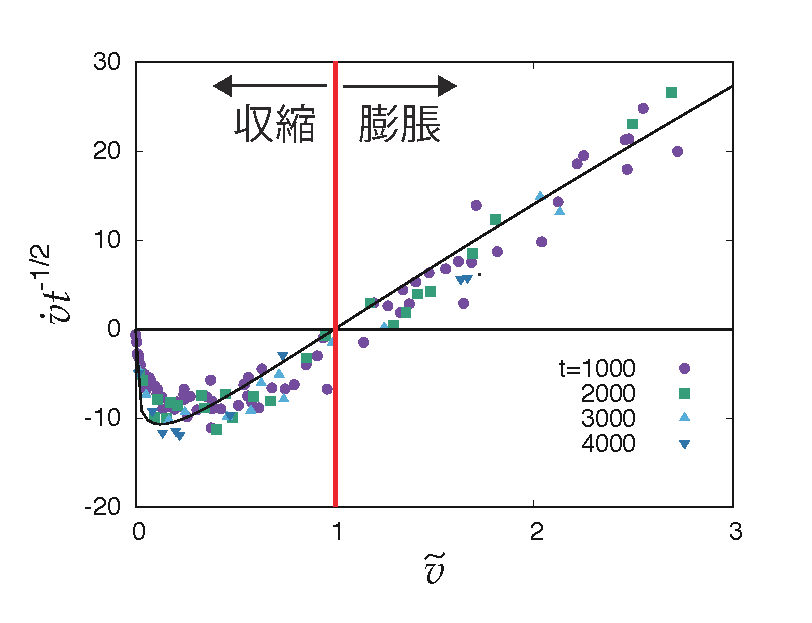
\includegraphics[width=0.9\linewidth]{vdot.pdf}
\caption{
気泡成長率のスケーリング.
ある時刻の気泡について,その体積と成長率の関係をプロットしており,
一つの点が一つの気泡に対応する.
異なる時刻における気泡成長率が単一の指数でスケールされており,理論曲線(実線)ともよく合うことがわかる\cite{Watanabe2016}.
}\label{fig_vdot}
\end{figure}

\section{プレスリリースとその反響について}

\begin{figure*}[bt]
\includegraphics[width=0.35\linewidth]{smithsonian.jpg}
\includegraphics[width=0.65\linewidth]{hpcwire.jpg}
\caption{
(左) Smithsonian Magazineの記事.タイトルは「The Physics of Champagne Bubbles Could Help Power the Future」.(右) HPCwireの記事.タイトルは「Champagne Ushers In New Year of Simulations for RIKEN」.
}
\end{figure*}

我々は得られた結果を論文にまとめ,米国物理学協会(American Institute of Physics, AIP)が出版する論文誌のひとつ,Journal of Chemical Physicsに投稿し,掲載されることになったのだが,AIPから我々の結果がプレスリリースされることになった.
やや科学的な話題からは外れるが,その経緯が興味深かったので少し紹介させていただきたい.
論文の掲載が決まった後,AIPに雇われたというサイエンスライターから,我々の成果がAIP outreachに選ばれ,
プレスリリースを書きたいからいくつか質問をさせて欲しい,というメールが届いた.
何度かそのサイエンスライターとメールのやりとりをした後,AIPのDirector of Media Servicesから
プレスリリースの最終稿が届いた.内容は我々の論文の成果を一般向けにわかりやすく解説したものであり,そのまま
掲載されるかと思っていたら,リリース直前になって件のDirectorから「タイトル少し盛ったから」というメールが届いた.
かくして我々の成果は「シャンパンの泡は世界のエネルギー危機を救う?(How the Physics of Champagne and Soda Bubbles May Help Address the World's Future Energy Needs)」という刺激的なタイトルでプレスリリースされた\cite{AIP}.
この記事の公開が12月で,欧米では新年をシャンパンで祝う風習があったことも影響したと思われるが,
このプレスリリースは大きな反響を呼んだ.すぐにスミソニアン博物館のウェブマガジン\cite{Smithsonian}を初めとする
いくつかのウェブサイトからメールによる取材があった.この話題はDiscovery Newsや,HPC Wire\cite{hpcwire}といった有名なサイトでも取り上げられ,それを参照したと思われるニュースサイトがさらにニュースを掲載,と多くのサイトに取り上げられた.
記事のタイトルも,最初は「エネルギー危機を救う?」だったが,シャンパンの泡が世界のエネルギー危機を解決する」「シャンパンの泡が世界のエネルギー工学を改革する」「シャンパンの泡があなたの家を照らす:科学者が語る」と,さながら伝言ゲームのように大げさになっていった.
果てはシャンパンやスパークリングワインを扱うオンラインショップが我々の論文を引用し「いつだってシャンパンが答えだってことはわかっていたことさ!」と言い出したり,「研究者はこの研究のために4000本のシャンパンを空けたそうだ.次のパーティには俺たちも呼んでくれよ.」などと,どうやら4000ノードの計算と4000本のシャンパンを取り違えたらしいニュースが掲載されるなど,対応に困る反響まであった.
言うまでもないことだが,我々の原著論文にはシャンパンという単語は全く入っていない.
一方,我々はAIPからプレスリリースの連絡を受けたあと,すぐに物性研でもプレスリリースしようとしたが,論文掲載までに時間がなかったために断念し,代わりに物性研ニュースなどで広報に努めたが,「渡辺宙志助教らが「京」による大規模気泡生成シミュレーションに成功」などというカタいタイトルがよくなかったためか,国内ではほとんどと言ってよいほど反響が無かった.

この一連の騒動は,研究のアウトリーチについて考える良い機会となった.特にタイトルのつけかた一つで,同じ論文に関する広報でも
こうも注目度が変わるものかと驚いた.無論,あまり実態とかけ離れたキャッチコピーをつけたり,誤解を招く広報は良くないが,
かといって正確さを優先させて無味乾燥なタイトルにしても広報の意味がない.
AIPが広報のために専任のDirectorを置き,さらにプレスリリースのためにサイエンスライターを雇って研究者とやりとりをして
リリース文を作る仕組みは大いに参考になった.

\section{おわりに}

我々は古典核生成論の平均場描像の妥当性検証のため,急減圧液体における気泡のオストワルド成長過程
の大規模計算を行った.その結果,気泡成長はオストワルド成長の古典論でよく記述されることがわかった.
これだけ相互作用が強い系において平均場描像が成立していることは大きな驚きであったが,
現在は気泡間相互作用のタイムスケールが気泡成長のタイムスケールよりも格段に早いため,
液滴成長とは逆の意味で平均場描像が正当化されると理解できる.
この計算には数億粒子規模の計算が求められるため,「京」のような大規模計算資源が必須であった.
私事で恐縮だが,私が博士課程の三年目の時,当時世界最高の性能を誇っていた地球シミュレータを
使うプロジェクトに参加する機会があった.しかし,当時は博士論文の執筆等で忙しく,
せっかくの世界最高の計算機をほとんど使うことができないまま,そのプロジェクトが終わってしまったのが心残りであった.
その時,「次の国策スパコンは絶対に使い倒してやる」と心に誓ったのを覚えている.
その悔しさから十余年,ようやくリベンジの機会が訪れ,「京」を使って成果を挙げることができ,感慨もひとしおである.
2013年当時,「京」でしかできなかった計算は,既に現在の物性研のスパコンで手が届く領域になっている.
スパコンは,ハードウェア,ソフトウェアともに発展が速く,これからもどんどんこれまで不可能と思われていたようなことができるように
なっていくであろう.筆者も大規模計算で初めて見える面白い物理を追究するとともに,その面白さを広める努力もしていきたい.

\section*{謝辞}
本研究は,九州大学(当時)の鈴木将氏,理研AICSの稲岡創氏,東大の伊藤伸泰氏との共同研究です.また論文をまとめるにあたり,
物性研の川島先生をはじめ,多くの方にご助言をいただきました.
本研究は,科学研究費補助金(No.~23740287)の補助を受けて行われました.
計算資源として理化学研究所の「京」(課題番号hp130047),及び物性研共同利用スパコンを使わせていただいております.
「京」の全系計算の実施においては,藤堂先生を始め,CMSI事務局の皆様,RISTの皆様に大変お世話になりました.
理研AICSの皆様には,研究成果の紹介などでお世話になりました.ここに深く感謝いたします.

\begin{thebibliography}{99}
\bibitem{Baldan} A. Baldan: J. Mater. Sci. \textbf{37}, (2002) 2171.
\bibitem{ice} C. Clark: \textit{The Science of Ice Cream} (Royal Society of Chemistry, 2004).
\bibitem{LS} I. Lifshitz and V. Slyozov: J. Phys. Chem. Solids \textbf{19}, (1961) 35.
\bibitem{Wagner} C. Wagner: Z. Elektrochem. \textbf{65}, (1961) 581
\bibitem{Gibbs} J. W. Gibbs: \textit{The Collected Works of J. W. Gibbs}, Vol I (Longmans, New York, 1928).
\bibitem{CNT} J. Feder, K. C. Russel, J. Lothe, and G. M. Pound, Adv. Phys. \textbf{15}, (1966) 111.
\bibitem{Horsch} M. Horsch, J. Vrabec, and H. Hasse: Phys. Rev. E \textbf{78}, (2008) 011603.
\bibitem{Vinogradov} V. E. Vinogradov, P. A. Pavlov, and V. G. Baidakov: J. Chem. Phys. \textbf{128}, (2008) 234508. 
\bibitem{Zeng} X. C. Zeng and David W. Oxtoby: J. Chem. Phys. \textbf{94}, (1991) 4472.
\bibitem{Yamamoto} T. Yamamoto and S. Ohnishi: Phys. Chem. Chem. Phys. \textbf{12}, (2010) 1033.
\bibitem{wtime} H. Watanabe, M. Suzuki, and N. Ito: Phys. Rev. E 82, (2010) 051604.
\bibitem{Farkas} L. Farkas: Z. Phys. Chem. \textbf{125}, (1927) 236.
\bibitem{Zeldovich} J. B. Zeldovich: J. Exp. Theor. Phys. \textbf{12}, (1942) 525.
\bibitem{Blander} M. Blander and J. L. Katz: AIChE. J, \textbf{21}, (1975) 833.
\bibitem{Binder} K. Binder: Phys. Rev. B 15, (1977) 4425.
\bibitem{mdacp} \url{http://mdacp.sourceforge.net/}
\bibitem{mdnote} H. Watanabe, M. Suzuki, and N. Ito: Prog. Theor. Phys. \textbf{126} (2011) 203-235.
\bibitem{fx10full}H. Watanabe, M. Suzuki, and N. Ito: Comput. Phys. Commun. \textbf{184}, (2013) 2775.
\bibitem{Watanabe2014} H. Watanabe, M. Suzuki, H. Inaoka, and N. Ito: J. Chem. Phys. \textbf{141} (2014) 234703.
\bibitem{Watanabe2016} H. Watanabe, H. Inaoka, and N. Ito: J. Chem. Phys. \textbf{145}, (2016) 124707.
\bibitem{AIP} \url{https://www.aip.org/publishing/journal-highlights/how-physics-champagne-and-soda-bubbles-may-help-address-worlds-future}
\bibitem{Smithsonian} \url{https://www.smithsonianmag.com/science-nature/new-years-physics-champagne-bubbles-could-help-power-future-180953778/}
\bibitem{hpcwire} \url{https://www.hpcwire.com/2015/01/07/champagne-ushers-new-year-simulations-riken/}
\end{thebibliography}

\end{document}
